\section{Time dependence and accuracy} \label{sec:ch:results:timeDependence}

In this section we present the measurement accuracy and its dependence on integration time.
The results presented here are the main results of the thesis.

\subsection{State preparation - heralding}

We found that the qubits had 5\%-8\% probability to be in the excited state when idling.
To remove this initialization error from characterization of the measurement process, we use heralding \cite{Johnson:heralding2012}.
Each pulse sequence begins with a measurement pulse, and only those experimental repetitions in which this first measurement pulse yields $\ket{0}$ are kept.
In this way, we effectively force the qubit into $\ket{0}$ at the start of each pulse sequence.
This heralding process brought the $\ket{0}$ preparation probability to $>99.3\%$, as we will see below.

\subsection{Fidelity at fixed measurement time}

Preparing the qubit into either $\ket{0}$ or $\ket{1}$, we inject a measurement pulse and digitize the scattered wave.
We kept trials for which demodulation of the heralding pulse yielded $\ket{0}$.
We then demodulated the measurement signal for 140\,ns, beginning at the start of the measurement pulse when there were nearly zero photons in the resonator.
This yielded two sets of IQ points, one for $\ket{0}$ and one for $\ket{1}$ as shown in Fig.\,\ref{Fig:ch:results:sec:timeDependence:IQPoints}.
As predicted in Ch.\,\ref{ch:DispersiveMeasurement}, the demodulated IQ points form two dimensional Gaussian distributions.
The finite separation and width of the distributions means that, with a single IQ measurement, we have a probability of erroneously identifying the qubit state.
We characterize the error in two ways: first using just the intrinsic signal to noise ratio of the dispersed photons, and second including non-ideal behavior of the qubit.

\subsubsection{Separation error}

We first characterize errors from the intrinsic signal to noise ratio of the dispersed photons.
This is captured by the separation error $\epsilon_\text{sep}$ defined in Ch.\,\ref{ch:DispersiveMeasurement}.
Projecting the two dimensional IQ distributions onto the line connecting their centers produces a pair of one dimensional Gaussian distributions, as shown in the inset of Fig.\,\ref{Fig:ch:results:sec:timeDependence:IQPoints}.
We find that the distributions are well fit by parabolas on the log scale, indicating good Gaussian shape.
From the fits, we compute $\epsilon_{\text{sep}}$ using Eq.\,(\ref{eq:sec:Lollipops:epsilon_sep}).
Here, we found $\epsilon_{\text{sep}} = 0.2\%$.

\begin{figure}
\begin{centering}
\includegraphics[width=\textwidth]{IQPoints.pdf}
\par\end{centering}
\caption{Measurement events for one qubit after 140\,ns pulse integration. Points in the wrong cluster are due to unwanted qubit state transitions. The appearance of more red points in the blue cluster than blue points in the red cluster is partially an artefact of the plot, and partially due to the fact that the qubit undergoes more downward transitions than upward transitions. The inset shows histograms of the IQ points projected onto the line connecting the centers of the $\ket{0}$ and $\ket{1}$ clouds. Heavy lines are Gaussian fits to the histograms are used for computing the separation error.}
\label{Fig:ch:results:sec:timeDependence:IQPoints}
\end{figure}

\subsubsection{State errors}

In the histogram shown in the inset of Fig.\,\ref{Fig:ch:results:sec:timeDependence:IQPoints}, we can see bins with counts greatly exceeding the parabolic fit.
For example, there are far more red counts at $x=-1$ than predicted by the red fit line.
These counts come from repetitions in which the qubit undergoes a state transition event before or during the measurement pulse.
A simple example is a qubit which undergoes a $T_1$ decay event near the beginning of the measurement pulse.
After the $T_1$ decay, the qubit is in $\ket{0}$, so the measured IQ point may be deep within the $\ket{0}$ cloud, but because that qubit was prepared as $\ket{1}$, we mark it as red.
Other sources of this type of error are $\ket{0} \rightarrow \ket{1}$ qubit transitions, improperly prepared states due to the finite accuracy of the heralding measurement pulse, and transitions induced by the measurement pulse itself.
We define the ``state errors'' $\epsilon_{\ket{0}}$ ($\epsilon_{\ket{1}}$) as the probability that a qubit nominally prepared in $\ket{0}$ ($\ket{1}$) is incorrectly identified.
We find $\epsilon_{\ket{0}}=0.7\%$ and $\epsilon_{\ket{1}}=1.3\%$.
These state errors are just at the $\sim 1\%$ threshold needed for the surface code.
Larger qubit $T_1$ values, accessible through use of MBE grown aluminum films \cite{Megrant:highQ2012} would improve $\epsilon_{\ket{1}}$.

\subsection{Time dependence}

While separation fidelity is improved by collecting more scattered photons, this requires longer measurement and thus incurs more qubit errors.
To fully characterize this trade-off, we varied the upper limit of the time integration used in extracting the IQ points, thus building a time series of $\ket{0}$ and $\ket{1}$ IQ clouds.
We plot the data in three dimensions, with time on the z-axis and with each x-y plane representing an IQ plane at a single time.
An example with the qubit prepared in $\ket{0}$, $\ket{1}$, and $\ket{2}$ is shown in Fig.\,\ref{Fig:ch:results:sec:timeDependence:worldLines}.
Each thread in the plot corresponds to a single repetition of the experiment, ie. a single measurement event.
At the beginning of the measurement pulse $t=0$, the branches for the three prepared states are indistinguishable.
At the beginning of the pulse, photons begin to be collected, but the resonator has not yet rung up, so the photons are not phase shifted.
During this time, the branches all move away from their starting position but remain clustered.
Once the resonator has rung up, the scattered photons carry information about the qubit state, and the branches begin to separate.
Integrating more signal and noise increases the separation and the widths of the branches.
%Figure \ref{Fig:ch:results:sec:timeDependence:IQPoints} represents a fixed time slice of Fig.\,\ref{Fig:ch:results:sec:timeDependence:worldLines}.

\begin{figure}
\begin{centering}
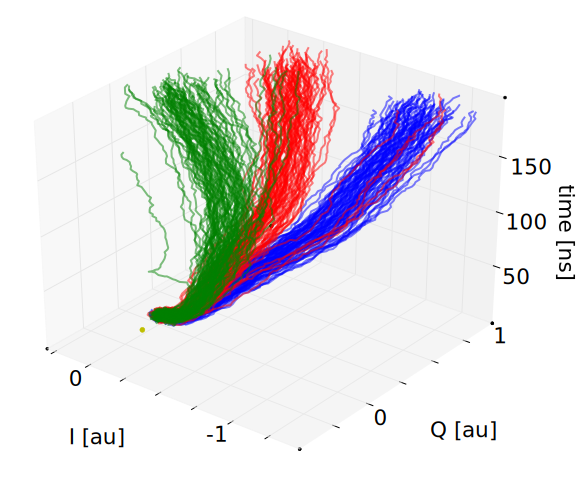
\includegraphics[width=\textwidth]{worldLines.pdf}
\par\end{centering}
\caption{IQ trajectories during integration of the measurement pulse, showing approximately 150 separate measurements.
The three branches correspond to the qubit prepared in the $\ket{0}$ (blue), $\ket{1}$ (red), or $\ket{2}$ (green) states.
Note the green threads which jump to the red branch part way through the measurement, which represent $\ket{2}\rightarrow\ket{1}$ qubit transitions.}
\label{Fig:ch:results:sec:timeDependence:worldLines}
\end{figure}

Next, we find the time dependent separation and state errors.
For each time slice during the measurement we construct IQ clouds as in Fig.\,\ref{Fig:ch:results:sec:timeDependence:IQPoints}.
Once we recorded the time domain traces $I(t)$ and $Q(t)$, we extracted the time dependent separation error $\epsilon_{\text{sep}}(t)$ at each $t$ in the same way as described above.
We then used the separation $\delta(t) \equiv \left| \langle I(t) \rangle - \langle Q(t) \rangle \right|$ as an optimal weighting window to re-integrate the data.
In other words, once we knew $\delta(t)$ we multiplied $I(t)$ and $Q(t)$ by $\delta(t)$ and re-integrated.
This emphasized the data where the IQ clouds for each state are better separated.
From the re-integrated data we extract $\epsilon_{\text{sep}}$, $\epsilon_{\ket{0}}$, and $\epsilon_{\ket{1}}$.
We wish to build a multiplexed system capable of measuring several qubits simultaneously, so we performed the experiment on two qubits, $Q_2$ and $Q_4$ at the same time, as shown in Fig.\,\ref{Fig:ch:results:sec:timeDependence:errorVsTime}.

\begin{figure}
\begin{centering}
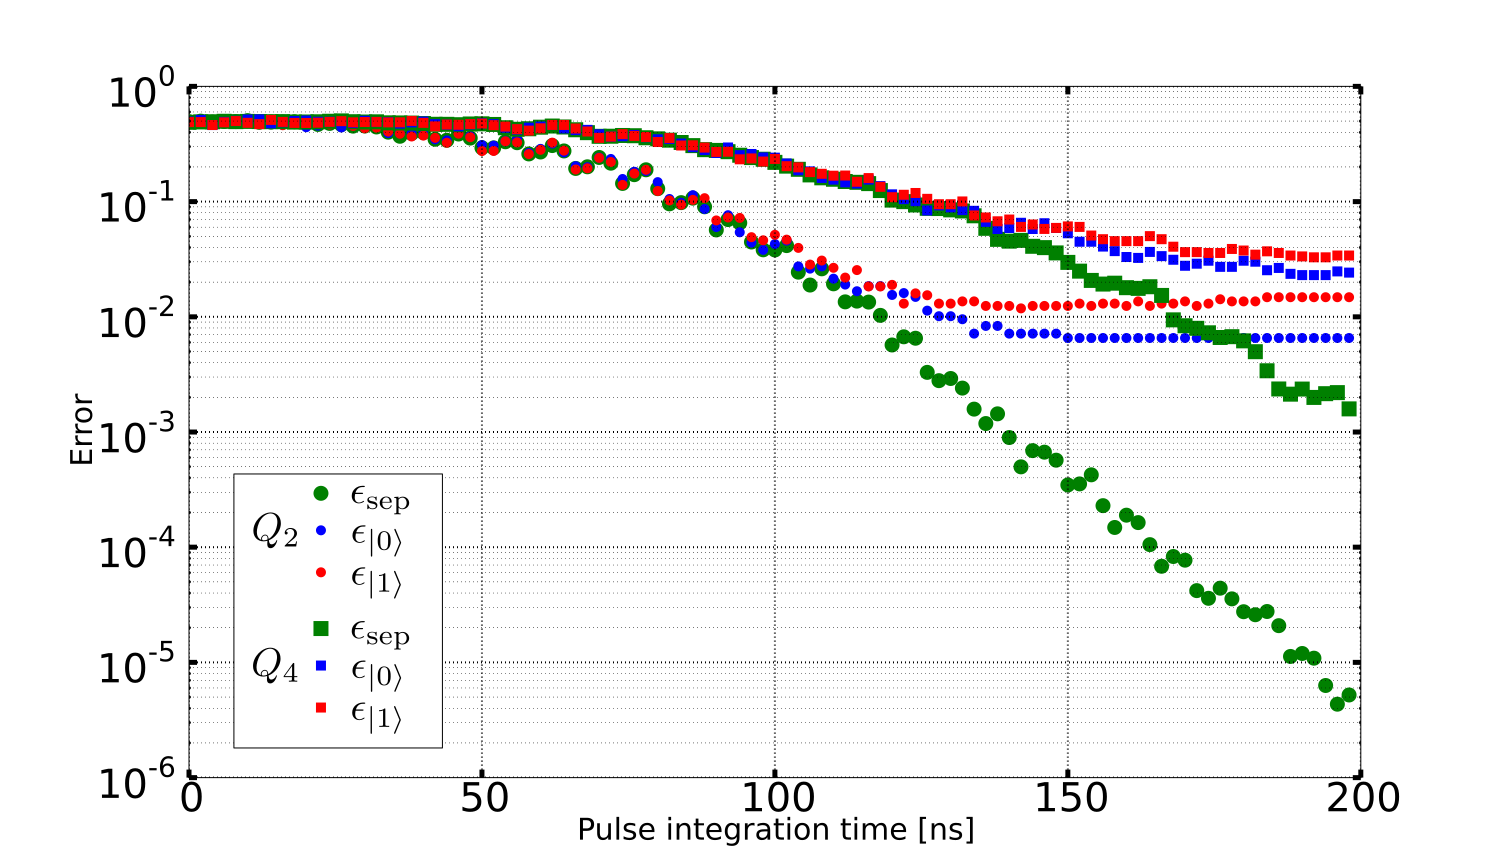
\includegraphics[width=\textwidth]{errorVsTime.pdf}
\par\end{centering}
\caption{Time dependence of measurement errors for qubits $Q_2$ (circles) and qubit $Q_4$ (squares) measured simultaneously. Green points indicate the separation error $\epsilon_{\text{sep}}$, while the blue and red points represent $\epsilon_{\ket{0}}$ and $\epsilon_{\ket{1}}$ respectively. The data in Fig.\,\ref{Fig:ch:results:sec:timeDependence:IQPoints} came from the $t=140\,\text{ns}$ point for $Q_2$.}
\label{Fig:ch:results:sec:timeDependence:errorVsTime}
\end{figure}

We focus first on the data for qubit $Q_2$. The separation error changes slowly with time for the first 50\,ns while the resonator rings up.
As shown in Fig.\,\ref{Fig:ch:results:sec:characterization:photonsVsTime}, the resonator photon occupation reaches the maximum value after approximately 50\,ns.
As the resonator photon number increases, the slope of $\epsilon_{\text{sep}}(t)$ increases until attaining a constant value at about 125\,ns of approximately one decade per 25\,ns.
The constant slope on the semi-log scale is consistent with Eq.\,(\ref{eq:sec:lollipops:e_sepVsSNR}).

The state errors decrease along with the separation error for the first 100\,ns, and then begin to saturate.
The saturation is explained by two deleterious qubit state transition processes.
We have measured that, in equilibrium, the qubits experience upward $\ket{0}\rightarrow\ket{1}$ transitions with a rate of $\Gamma_{\uparrow}\approx 1/100\,\mu\text{s}$, which result in excited state populations of 5\% to 8\%.
These transitions lead to state preparation errors; with 500\,ns between the heralding and final measurements, we expect 0.5\% re-population of the excited state before the start of the final measurement.
This nearly explains the saturation of $\epsilon_{\ket{0}}$ at 99.3\%.
The second error process is the usual qubit energy relaxation; a qubit transition before the halfway point of the measurement leads to an error.
With a measurement time of 140\,ns and $T_1=10\,\mu\text{s}$ we expect an extra 0.7\% loss in excited state population, yielding an expected limit of 98.8\%.
This agrees well with the measured $\epsilon_{\ket{1}}$ saturation at 98.7\%.

The separation fidelity for $Q_4$ is qualitatively similar to the data for $Q_2$, but with slower approach to the constant slope region.
Qubit $Q_4$ is slower because it has $\kappa_r^{-1}=147\,\text{ns}$, which is slower for $Q_2$ where $\kappa_r^{-1}=37\,\text{ns}$.

These data demonstrate the viability of multiplexed, dispersive state measurement.
In particular, the qubit with fast $\kappa_r$ approaches 99\% accuracy for the state errors in this multiplexed measurement.

As the more aggressive $\kappa_r$ used in qubit $Q_2$ did not produce a measurable suppression in $T_1$, future designs should use even faster values of $\kappa_r$.
The qubit with the most aggressive $\kappa_r$ in the present experiment, $Q_1$, could not be carefully characterized because of the error which placed $Q_3$'s measurement resonator too close in frequency to $Q_1$'s measurement resonator.

\subsection{Multiplexed measurement}

We measured all four qubits simultaneously, as shown in Fig.\,\ref{Fig:ch:results:sec:timeDependence:fourQubitMultiplexed}.
Three of the four qubits, $Q_1$, $Q_2$, and $Q_3$, reached $\epsilon_{\text{sep}}<1\%$ within 200\,ns.
The fourth device, $Q_4$, which had the most conservative $\kappa_r T_1$ product, reached $\epsilon_{\text{sep}}=1\%$ in 266\,ns.
In order to prevent saturation of the parametric amplifier while simultaneously measuring all four devices, we reduced the drive powers relative to the two qubit case discussed previously.
This lead to lower SNR and accordingly required longer integration time, which is why the time for eg. $Q_2$ to reach $\epsilon_{\text{sep}}=1\%$ is longer here than in Fig.\ref{Fig:ch:results:sec:timeDependence:errorVsTime}.

For qubits $Q_2$ and $Q_4$ the performance is nearly as good as for the two qubit case.
The small degradation of performance comes from increased qubit transitions during the longer measurement time.
Qubits $Q_1$ and $Q_3$ show higher $\epsilon_{\ket{1}}$.
As shown in the inset of Fig.\,\ref{Fig:ch:results:sec:characterization:resonatorDips} the measurement resonators for qubits $Q_1$ and $Q_3$ are closely spaced in frequency (13 MHz).
This close spacing adversely affects the frequency discrimination step of the measurement via spectral leakage, leading to increased measurement error.
This is seen in Fig.\,\ref{Fig:ch:results:sec:timeDependence:fourQubitMultiplexed} where the $\epsilon_{\text{sep}}(t)$ for $Q_3$ does not follow a line on the semi-log plot.
More importantly, the measurement photons induce large qubit frequency shifts (200\,MHz to 300\,MHz) via the ac Stark effect, as shown in Fig.\,\ref{Fig:ch:results:sec:characterization:photonsVsTime}.
This causes the qubits to cross through resonance with material defects and lose $\ket{1}$ population.
This was the main cause of the poor $\epsilon_{\ket{1}}$ on $Q_1$.
We were able to mostly work around this problem with careful choice of operating frequency in qubits $Q_2$, $Q_3$, and $Q_4$, but limited total available frequency space led to degraded performance in $Q_1$ which was tuned up last.
This problem would be substantially mitigated in devices constructed with epitaxial Al films grown on plasma cleaned substrates as, this was shown to significantly reduce the number and coupling strengths of the defects \cite{Megrant:highQ2012}.

\begin{figure}
\begin{centering}
\includegraphics[width=\textwidth]{fourQubitMultiplexed.pdf}
\par\end{centering}
\caption{Simultaneous measurement of four qubits. Separation (green) and state (blue and red) fidelities are shown similarly to Fig.\,\ref{Fig:ch:results:sec:timeDependence:errorVsTime}.
Ripples on qubits $Q_1$ and $Q_3$ were caused by spectral leakage.}
\label{Fig:ch:results:sec:timeDependence:fourQubitMultiplexed}
\end{figure}
